\documentclass[conference,compsoc]{report}
\usepackage{graphicx} 
\ifCLASSOPTIONcompsoc
  % IEEE Computer Society needs nocompress option
  \usepackage[nocompress]{cite}
\else
  \usepackage{cite}
\fi

\ifCLASSINFOpdf
\else
\fi
\hyphenation{op-tical net-works semi-conduc-tor}

\begin{document}

\title{Report of ASC Student Supercomputer Challenge 2017 Preliminary Contest}

\author{\IEEEauthorblockN{Zhibin Xie, Zhen'ning Wang, Jiafang Xue, Guohua Tian}
\IEEEauthorblockA{School of Information Engineering,\\ NanChang University}

\and

\IEEEauthorblockN{Xianling Dong}
\IEEEauthorblockA{School of Science,\\NanChang University}

}

\maketitle

\begin{abstract}
-- NSBSS.
\end{abstract}
\IEEEpeerreviewmaketitle

\section{Introduction}
We are a group of youths loving computer science who have a
huge dream, and working hard for reaching higher. We gathered
together due to strong interest in supercomputer.

\hfill NSBSS
 
\hfill March 5, 2017

\subsection{Team's Information}
NSBSS Team is ASC Team of NanChang University...


\subsection{Other Informations}
etc.

% ------HPL Test------

\section{HPL Test}
% Details of HPL Test, such as MAX score, config and so on...\\
% I wish you the best of success.
1) HPL install \\

In this test and optimize, we chose Intel® Optimized LINPACK. \\

2) Test Step \\

2.1) PxQ \\

Because Intel® Optimized LINPACK use all CPU core in multi-thread
by default, so we set P x Q to 1 x 1. \\

2.2) BLAS \\
There are many blas, such as openblas, mkl, gogoblas and atlas.
Because we are using intel xeon phi, MKL will be the best choice \\

2.3) N \\
Experience tells us, N can be calculated by 
\[ N^2 * 8 = MEM * 80\% \]

so N should have been  82900, but in our test, when N is set to \\
35000, GFlops reach to 1.7GFlops, which is much higher when N is 829000 \\

\begin{tabular}{|c|c|c|c|c|c|c|}
\hline
N &  33000 & 34000 & 35000 & 36000 & 37000  \\
\hline
GFlops  &1702 &1701.48 &1714.1 &1708.11 &1501.21 \\
\hline
Time (S) &14.08 &15.4 &16.68 &18.21 &22.5 \\
\hline 
\end{tabular}
\newline
\newline
\par
2.4) NB \\
\par
\begin{tabular}{|c|c|c|c|}
\hline
NB & 232 & 256 & 296 \\
\hline
GFlops & 1709.86 & 1714.1 & 1702.39 \\
\hline
\end{tabular}

\subsection{Best Score}
Finally, we reached at 1.7Gflops. 
\subsection{Problems}
Problems we had meet here.

\subsection{etc.}
Subsection text here.

% ------MASNUM_WAVE------

\section{MASNUM\_WAVE}
% no \IEEEPARstart
Details of MASNUM\_WAVE, 2 line at least....\\
line.2

\subsection{Information I}
Subsection text here.

\subsection{Information II}
Subsection text here.

% ------PaddlePaddle------

\section{Deep learning contest}
In-depth learning is a learning algorithm that simulates the cognitive pattern of the human brain, and the current Baidu Research Institute uses the strategic direction of data mining and artificial intelligence as an important development strategy of the 21st century.

PaddlePaddle is originated in Baidu's open source depth learning platform.And it's easy to use.

\subsection{Analysis of the problem}
Data are sampled from mobile phone APP.Using the dataset which are aggregated about 50 days from 00:00 a.m. on March 1st to 08:00 on April 20th for training. Your task is to predict each link's speed for every 5 minutes from 08:00 to 10:00 on April 20th.

The model outputs are evaluated by the Root Mean Squared Error (RMSE) of
predictions.

$$RMSE = \sqrt{\frac{ \sum_{i=1}^{n} \left ({X}_{actual, i} - {X}_{model, i} \right )^{2}}{n} }$$

\footnote A ${X}_{actual, i}$ is actual value of moment i, while ${X}_{model, i}$,i is your prediction moment of i
\\
\\
By simply observing the node graphs, we map the traffic nodes, for example, simple crossroads

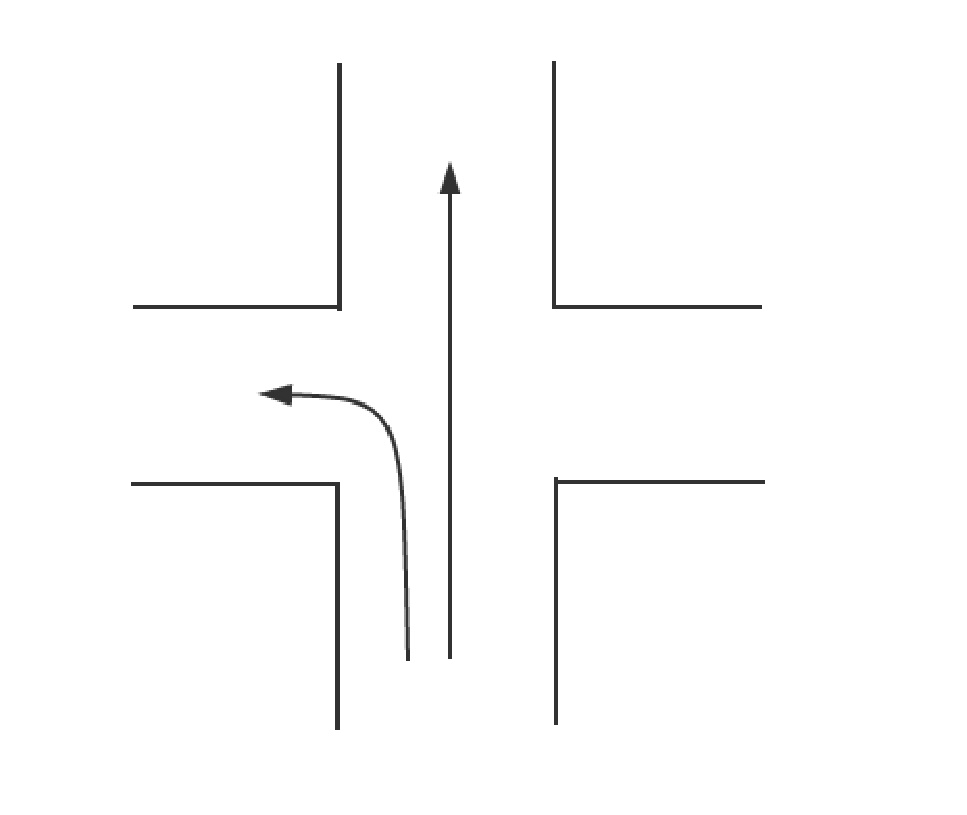
\includegraphics[width=3.00in,height=2.00in]{crossroads.eps}

Corresponding to the four traffic states.

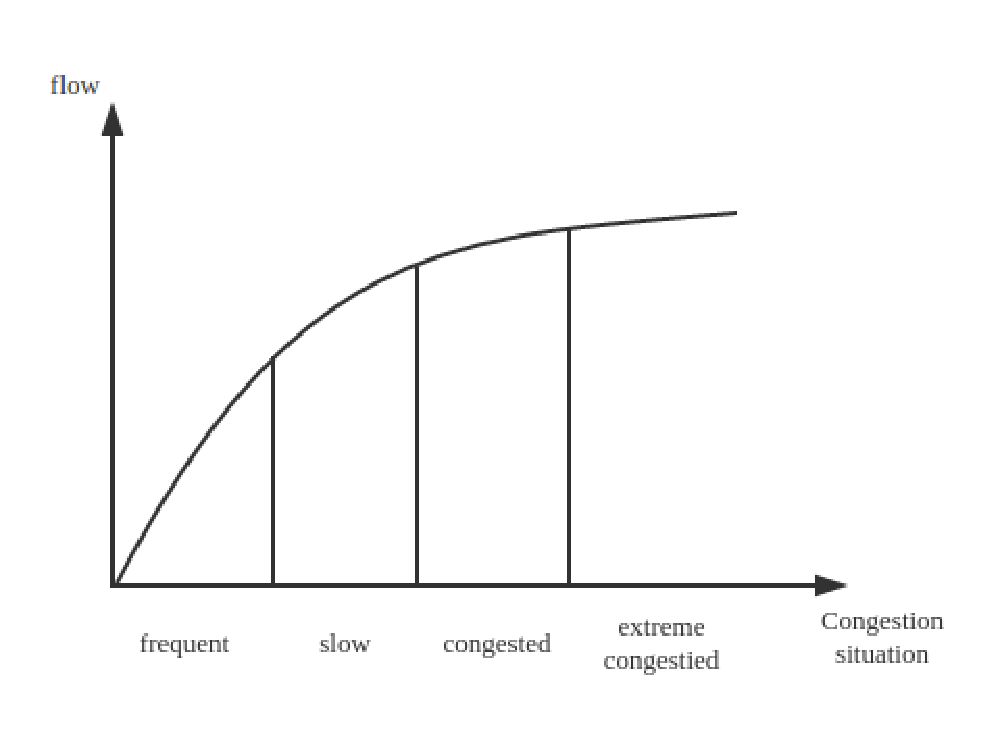
\includegraphics[width=3.00in,height=2.00in]{states.eps}

The result of clustering is the four eigenvectors (1, 2, 3, 4) corresponding to the state defined by the topic. The four eigenvectors represent smooth, slow, crowded and very crowded.

\subsection{Questions}
After we downloaded the data, we found that the amount of data is large, some of the data there is a large interference, so the data processing is very important.We also have little understanding of the depth of learning. so it is difficult to find theoretical support.
And the results of the prediction, and the calculation is unclear.


\subsection{Preliminary solution}
\subsubsection{Data processing}
Through the analysis of the title and data, we selected the daily time from 00:00-02:00, 04:00-06:00, 08:00-10:00, 12:00-14:00, 16:00-18:00 and 20:00-22:00 six time periods as the representative.In order to reduce the error, we take the average of the time to process the data.

\subsubsection{Algorithm selection}
Algorithm we used RMSProp, RMSProp is a very efficient algorithm, RMSProp slightly improved AdaGrad, making the algorithm no longer as radical as AdaGrad it is moving average of squared gradients.
\\
\\
The equations of this method as follows:

$$ \nu\left (w, t \right ) = \rho \nu\left ( w, t - 1 \right ) + \left ( 1 - \rho \right )\left ( 
\nabla{Q}_{i}(w) \right )$$

$$ w  = w - \frac{\eta }{\sqrt{\nu (w, t) + \varepsilon }} \left ( \nabla{Q}_{i}(w) \right )$$

\subsubsection{Result analysis}
We perform the error analysis by plotting the original data, and comparing the resulting data
\\
\\
Relative error:
$$ rerr = \frac{{X}_{actual, i} - {X}_{model, i}}{{X}_{actual, i}} $$
\\
\\
Absolute relative error:
$$ mrerr = \frac{1}{N} \sum_{1}^{N}\left ( \frac{{X}_{actual, i} - {X}_{model, i}}{{X}_{actual, i}} \right ) $$


\subsection{Algorithm improvement}
Adam is a recently proposed algorithm that is similar to the RMSprop comparison with the momentum. The procedure is similar to:


$$m(w,t) = {\beta}_{1} m(w, t - 1) + (1 - {\beta}_{1})\nabla{Q}_{i}(w)$$
$$v(w,t) = {\beta}_{2} v(w, t - 1) + (1 - {\beta}_{2})(\nabla{Q}_{i}(w))^{2}$$
$$w  = w - \frac{\eta }{\sqrt{\nu (w, t) + \varepsilon }}$$

And we set eps=1e-6, bata1=0.9, beta2=0.999.


\subsection{Parameter configuration}
Choose a suitable learning rate is very difficult, in the beginning, we set the way through the schedule learning learning method, that is pre-designed a certain series of iterations to increase or increase learning rate.As the learning rate increases, we find that the relative error begins to increase.Finally we set the learning rate to 1e-6.

% -----Conclusion-----

\section{Conclusion}
No conclusion yet...

% ----Appendix-----

\section{Appendix}
No appendix yet.

\subsection{A.}
Appendix A.


% ---- References----

\begin{thebibliography}{1}

\bibitem{IEEEhowto:kopka}
%H.~Kopka and P.~W. Daly, \emph{A Guide to \LaTeX}, 3rd~ed.\hskip 1em plus
%  0.5em minus 0.4em\relax Harlow, England: Addison-Wesley, 1999.\\
  
 
No reference yet...

\end{thebibliography}

\end{document}


